\documentclass{article}
\usepackage[utf8]{inputenc}
\usepackage{amsmath}
\usepackage{graphicx}
\vspace*{1cm}

   \textbf{University of Science - HCMUS}

   \vspace{0.5cm}
    CSC15106 – Knowledge Engineering Seminar

\vspace{1.5cm}

\title{Lab 01: Hybrid Encryption}
\author{21120263 - Tong Nguyen Minh Khang}
\date{\today}

\begin{document}

\maketitle

\section{Introduction}
This report describes a simple hybrid encryption system for secure file exchange.

\section{System Overview}
The system consists of the following main components:
\begin{figure}[h]
    \centering
    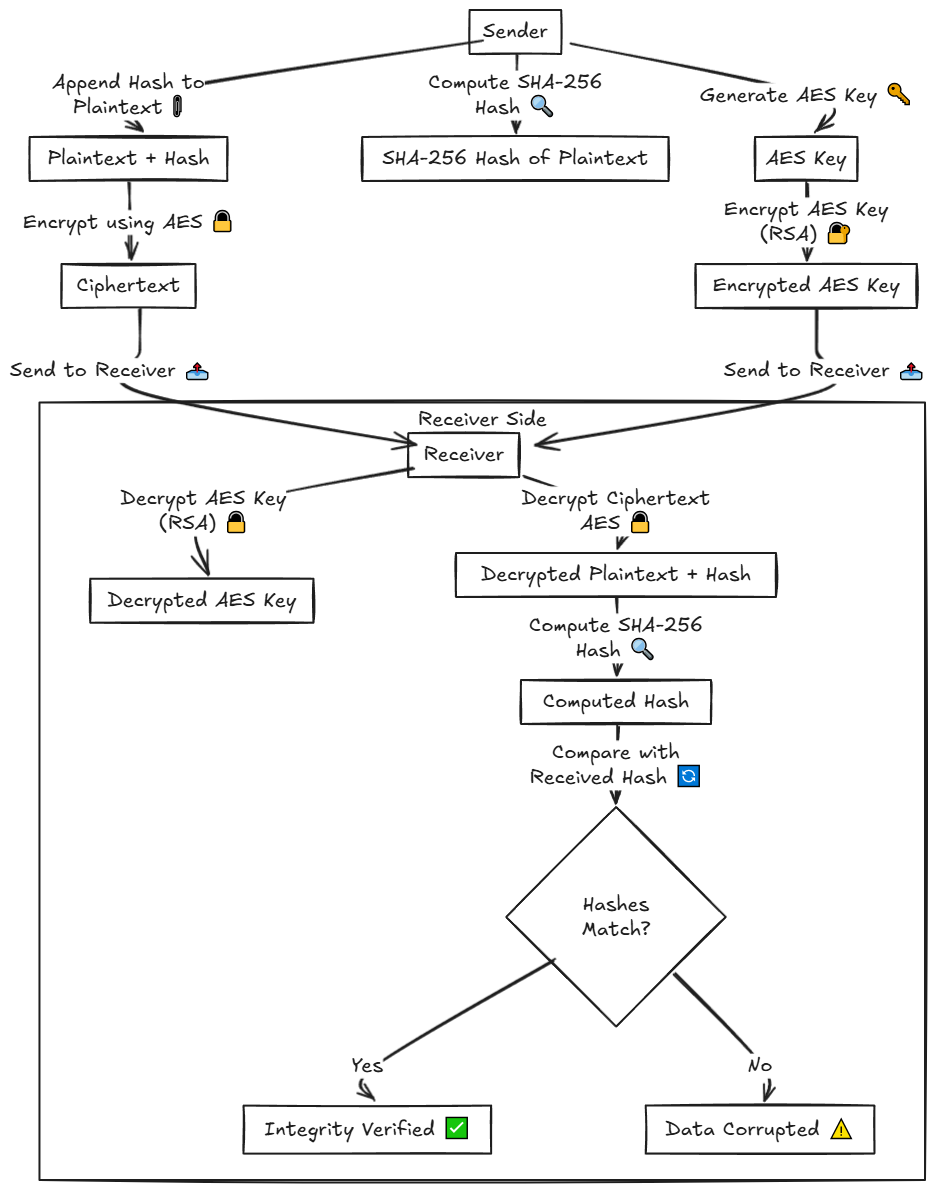
\includegraphics[width=0.5\textwidth]{diagram.png}
    \caption{This is a caption for the image.}
    \label{fig:sample}
\end{figure}

\begin{itemize}
    \item \textbf{RSA Encryption:} Used to encrypt the symmetric AES key.
    \item \textbf{AES Encryption:} Used for the encryption of the actual file data.
    \item \textbf{Hashing using SHA-256:} Applied to ensure data integrity by checking the hash of the encrypted file against that of the decrypted file. 


\section{Special Parameters}
The following parameters are notable in the encryption settings:
\begin{itemize}
    \item \textbf{RSA Key Size:} A standard of 2048 bits is used for generating RSA key pairs, providing a good balance between security and performance.
    \item \textbf{AES Key Size:} An AES block size of 16 bytes (128 bits) is utilized for encrypting the data.
    \item \textbf{Hash Algorithm:} The SHA-256 hash function is employed to verify the integrity of the encrypted data.
    \item \textbf{Supported File Types:} The system is designed to handle various binary files for encryption and decryption, with no explicit limitations on file types within the binary format.
\end{itemize}

\section{Conclusion}
The hybrid encryption system effectively combines the benefits of RSA and AES to ensure secure communication, data confidentiality, and integrity.

\end{document}